\newpage
\section{Questão 12-39}

\begin{figure}[H]
	\centering
	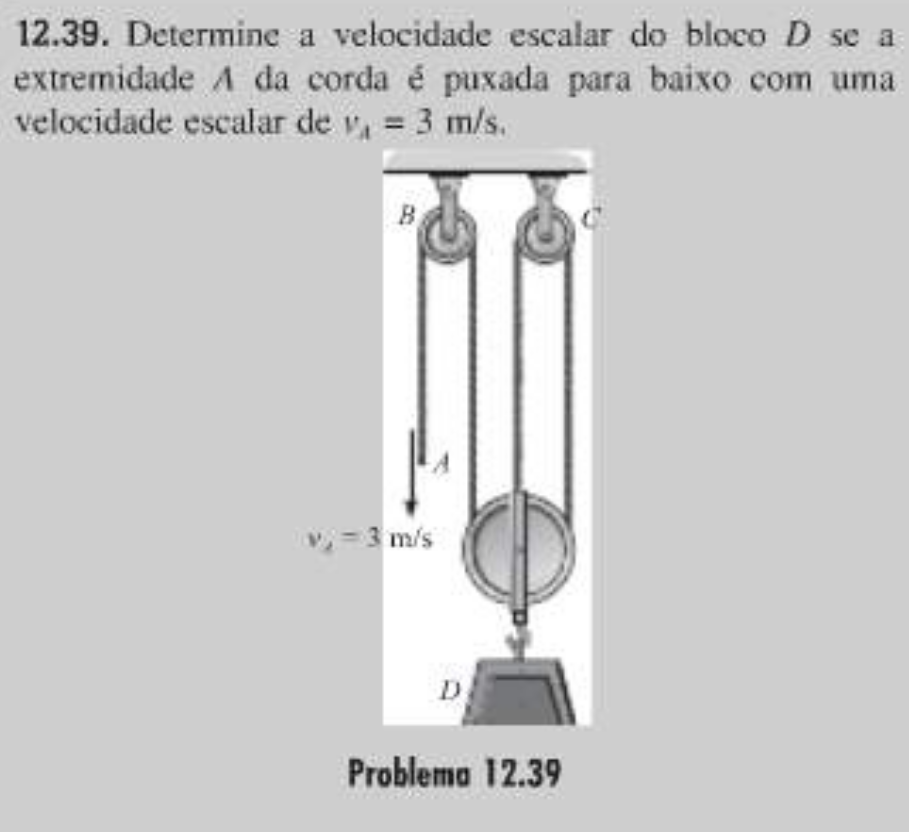
\includegraphics[width=.6\linewidth]{fundamentais/12-39.png}
	\caption{Comando da questão 12-39.}\label{fig:12-39}
\end{figure}

Nesta questão, analisamos um sistema de polias em que a velocidade de um ponto \(A\) é relacionada à velocidade de um bloco \(D\) devido à configuração do sistema de cordas. Determinamos a velocidade de \(D\) (\(v_D\)) quando a velocidade de \(A\) (\(v_A\)) é \(3 \, \text{m/s}\).

\subsection*{Relação entre as Velocidades}
No sistema de polias, podemos tratar os cabos como vetores de posição para identificar as velocidades relacionadas a cada elemento da seguinte forma:
\[
l_{\text{total}} = 3s_D + s_A
\]
onde:
\begin{itemize}
    \item \(s_A\): Cabo de comprimento BA, com referencial em \(A\);
    \item \(s_D\): Cabo de comprimento CD, com referencial em  \(C\).
\end{itemize}

Queremos identificar o quão rápido D se aproxima do ponto C quando A desce em uma velocidade de \(3\, m/s\), logo:
\subsection*{Cálculo de \(v_D\)}
Substituímos \(v_A = 3 \, \text{m/s}\) na equação:
\[
\frac{d \left(l_{\text{total}} = 3s_D + s_A\right)}{dt} \rightarrow 0 = 3v_D + v_A
\]

Resolvendo para \(v_D\):
\[
3_v_D + 3 \, \text{m/s} \rightarrow v_D = 1.0 \, \text{m/s}.
\]
